\noindent Die Rekursionsgleichungen können wir nun zur Formulierung des Pseudocodes für den Schaltkreis der tatsächlichen Überträge nutzen:

\begin{algorithm}[h!]
\caption{Berechnung der eigentlichen Überträge im CLA-Addierer.}
\begin{algorithmic}
\FOR{$l:= L-1$ \algto $0$}
\FOR{$i:= 1$ \algto $\frac{n}{2^l}$ \algpar}
\STATE  $c_{2i+1,l} = c_{i,l+1}$;
\STATE  $c_{2i,l} = g_{2i,l} \lor \left( c_{i-1,l+1} \land p_{2i,l} \right)$;
\ENDFOR
\ENDFOR
\end{algorithmic}
\end{algorithm}

\noindent Die innere \textbf{for}-Schleife braucht $O(1)$ Zeit, da sie vollständig parallel ausgeführt wird. Die äußere \textbf{for}-Schleife braucht $O(\log n)$ Zeit. Also ergeben sich für die Überträge folgende Größen:

\begin{eqnarray*}
\text{Tiefe: }T(n) & = & \log n \\
\text{Größe: }G(n) & = & \sum_{l=0}^{L-1}{\sum_{i=1}^{\frac{n}{2^l}}{O(1)}} = O(n)
\end{eqnarray*}

\noindent Mit den Überträgen können wir nun die endgültige Summe berechnen. Dabei bezeichnet $s_j$ die Summe an der Stelle $j$, mit $0 \leq j \leq n$, und $c_j = c_{i,l}$ den Übertrag an der Stelle $j$, mit $j = (2i+1)2^l-1$.

\begin{algorithm}[h!]
\caption{Berechnung der Summe.}
\begin{algorithmic}
\FOR{$j:= 0$ \algto $n-1$ \algpar}
\STATE  $s_j = a_j \oplus b_j \oplus c_j$;
\ENDFOR
\end{algorithmic}
\end{algorithm}

\noindent Hiermit werden alle Stellen der Summe, bis auf die Letzte ($n$-te Stelle), ausgerechnet. Sind wir  ebenfalls an dieser Stelle interessiert, so kann diese einfach durch $s_n = c_n$ berechnet werden. Das berechnen der Summe benötigt $O(1)$ Zeit; der zugehörige Schaltkreis ist $O(n)$ groß.\\
Damit ergeben sich für die insgesamte Tiefe und Größe des CLA-Addierers:
\begin{eqnarray*}
\text{Tiefe: }T(n) & = & \log n \\
\text{Größe: }G(n) & = & O(n)
\end{eqnarray*}

\pagebreak

\section{Überblick zur Vorlesung}
Die Vorlesung wird nach aktueller Planung folgende Themen ansprechen:

\begin{itemize}
\item Einleitung
\item Rechnermodelle
\item Elementare Techniken in parallelen Algorithmen
\item Suchen und Sortieren
\item Graphen
\item Strings
\item Arithmetik
\item Parallele Komplexitätstheorie
\end{itemize}

\section{Literatur}
\begin{description}
\item[S. Aki] The design and analysis of parallel algorithms
\item[J. Ja' Ja'] Introduction to parallel algorithms
\item[F.T. Leighton] Introduction to Parallel Algorithms and Architectures
\item[Cormen et. al.] Introduction to Algorithms, Kapitel 27, 3. Auflage
\end{description}

\chapter{Berechnungsmodell}
\newpage

\section{Klassifikation nach Flynn (1972)}
Nach Flynn können wir Rechnerarchitekturen wie folgt in grundlegende Klassen einteilen:

\begin{center}
\{ single, multiple \} instruction \{ single, multiple \} data
\end{center}

Daraus ergeben sich die nachfolgenden vier Architekturen:

\begin{description}
\item[SISD] Single Instruction, Single  Data \\
Diese Klasse enthält alle sequentiellen Einprozessor-Rechnerarchitekturen, wie z.B. Einprozessor-PCs: Hier wird nacheinander eine Operation auf ein einzelnes Datum angewandt.
\item[SIMD] Single Instruction, Multiple Data \\
Diese Architektur enthält Architekturen, bei denen eine Operationen auf viele Daten gleichzeitig angewendet werden kann. Dies trifft zum Beispiel auf sog. Vektorrechner oder die parallelen Berechnungseinheiten einer GPU zu.
\item[MISD] Multiple Instruction, Single Data \\
Sehr unintuitive Klasse; hier werden mehrere Operationen auf dasselbe Datum angewendet. Diese Architektur findet man bei special-purpose-Systemen, z.B. bei redundanter Berechnung zur Erhöhung der Fehlertoleranz.
\item[MIMD] Multiple Instruction Multiple Data \\
MIMD beinhaltet den Aufbau von Rechnernetzen bzw. verteilten Systemen, in denen allgemeine Threads/Prozesse modelliert werden können. Hier können verschiedene Operationen auf viele Daten vollparallel berechnet werden.
\end{description}

In der Vorlesung werden wir ein MIMD-artiges theoretisches Modell für parallele Algorithmen, die \textbf{PRAM}, nutzen. Die \textbf{PRAM} (\textbf{P}arallel \textbf{R}andom \textbf{A}ccess \textbf{M}achine) besitzt beliebig viele Prozessoren, die jeweils auf einen unendlich großen Speicher zugreifen (lesen und schreiben) können. Dabei benötigt jeder Schritt genau eine Zeiteinheit, explizite Synchonisierung wird nicht benötigt.

\begin{figure}[h!]
\centering
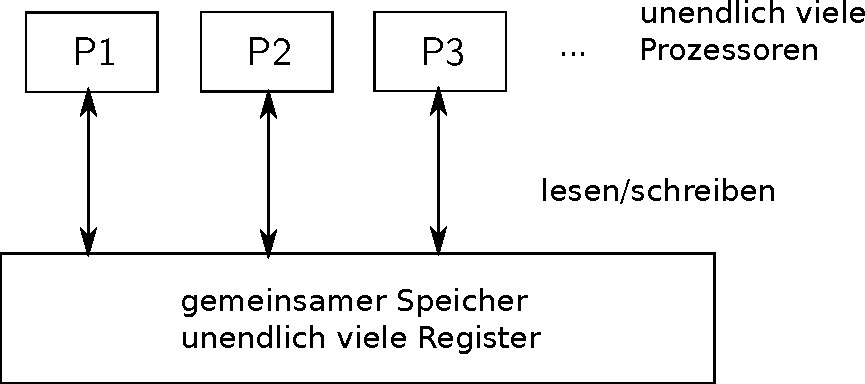
\includegraphics[scale=0.6]{bilder/pram.pdf}
\caption{Schematische Darstellung einer PRAM}
\end{figure}

Der Befehlssatz ist analog zu denen der "normalen" Registermaschine, beinhaltet also lesen, schreiben, verschiede arithmetische und Vergleichsoperationen.

\section{Lese- und Schreibzugriff}
Zusätzlich zur Architektur können wir auch das Verhalten bzgl. parallelem Zugriff auf gleiche Register im gemeinsamen Speicher unterscheiden:

\begin{center}
\{ \textbf{E}xclusive, \textbf{C}oncurrent \} \textbf{R}ead \{ \textbf{E}xclusive, \textbf{C}oncurrent \} \textbf{W}rite
\end{center}

Also können wir vier Abstraktionen unterscheiden:

\begin{enumerate}
\item EREW
\item CREW
\item ERCW
\item CRCW
\end{enumerate}

Bei der Abstraktion CRCW unterscheidet man drei Verhaltensweisen bei gleichzeitigem Schreibzugriff auf dasselbe Register:

\begin{description}
\item[beliebig] (engl. \emph{arbitrary}): Keine Kontrolle, wer schreibt.
\item[übereinstimmend] (engl. \emph{common}): Schreiben nur dann erfolgreich, wenn alle dasselbe schreiben.
\item[vorrangig] (engl. \emph{priority}): Prozessor mit kleinerem Index schreibt.
\end{description}

\newpage
\section{Ressourcen/Komplexitätsmaße}
Im Gegensatz zur sequentiellen Registermaschine können bei der \textbf{PRAM} zusätzliche Ressourcen gemessen werden.\\
Man unterscheidet:

\begin{description}
\item[(parallele) Laufzeit] bezeichnet die maximale Befehlsanzahl, die ein Prozessor ausführt.
\item[Zahl d. Prozessoren] die aktiv werden.
\item[Speicherplatz] bezeichnet die Anzahl der benutzen Register.
\item[Gesamtaufwand] (engl. \emph{work}) ist die Summe der Befehle pro Prozessor und kann durch das Produkt Laufzeit $\cdot$ Zahl d. Prozessoren abgeschätzt werden. 
\end{description}

\noindent Wie üblich wird der Ressourcenverbrauch als Funktion in der Größe der Eingabe angegeben. So betrachten wir als worst-case-Komplexität das Maximum und als durchschnittliche Komplexität den Mittelwert des ressourcenverbrauchs über alle Eingaben der Eingabegröße.

\noindent Als Funktionsnamen verwenden wir
\begin{eqnarray*}
T(n) & \text{für} & \text{Zeit} \\
P(n) & \text{für} & \text{Prozessoren} \\
S(n) & \text{für} & \text{Speicher} \\
W(n) & \text{für} & \text{Aufwand} 
\end{eqnarray*}

